\documentclass{article}

\usepackage{graphicx}
\usepackage{rotating}
\usepackage{amsmath}
\usepackage{amssymb}
\usepackage{mathrsfs}
\usepackage{fancyhdr}
\usepackage{listings}
\usepackage{xcolor}
\usepackage{color}
\usepackage{amsfonts}
\usepackage{textcomp}
\usepackage{float}
\usepackage{neuralnetwork}
\usepackage{pgfplots}
\usepackage[sorting=none]{biblatex}
\usepackage[margin=1in]{geometry}
\usepackage[font={small,it}]{caption}
\usepackage{placeins}
\usepackage{tikz}
\usepackage{xepersian}

%\usepackage[left=2cm,right=2cm,top=2cm,bottom=2cm]{geometry}


\usetikzlibrary{decorations.pathreplacing}
\usetikzlibrary{fadings}

\pgfplotsset{width=8cm,compat=1.17}

%\DeclareMathOperator*{\btie}{\bowtie}
\addbibresource{bibliography.bib}
\settextfont[Scale=1.2]{B-NAZANIN.TTF}
\setlatintextfont[Scale=1]{Times New Roman}
\renewcommand{\baselinestretch}{1.5}
\pagestyle{fancy}
\fancyhf{}
\rhead{تکلیف سوم درس یادگیری عمیق}
\lhead{\thepage}
\rfoot{علیرضا ابره فروش}
\lfoot{9816603}
\renewcommand{\headrulewidth}{1pt}
\renewcommand{\footrulewidth}{1pt}
\newcommand{\Lagr}{\mathcal{L}}
\newcommand{\Mod}[1]{\ (\mathrm{mod}\ #1)}
%%%%%%%%%%
\lstset
{
    language=[latex]tex,
    basicstyle=\ttfamily,
    commentstyle=\color{black},
    columns=fullflexible,
    keepspaces=true,
    upquote=true,
    showstringspaces=false,
    morestring=[s]\\\%,
    stringstyle=\color{black},
}
%%%%%%%%%%
%beginMatlab
\definecolor{mygreen}{RGB}{28,172,0} % color values Red, Green, Blue
\definecolor{mylilas}{RGB}{170,55,241}
%endMatlab
\begin{document}
%beginMatlab
\lstset{language=Matlab,%
    %basicstyle=\color{red},
    breaklines=true,%
    morekeywords={matlab2tikz},
    keywordstyle=\color{blue},%
    morekeywords=[2]{1}, keywordstyle=[2]{\color{black}},
    identifierstyle=\color{black},%
    stringstyle=\color{mylilas},
    commentstyle=\color{mygreen},%
    showstringspaces=false,%without this there will be a symbol in the places where there is a space
    numbers=left,%
    numberstyle={\tiny \color{black}},% size of the numbers
    numbersep=9pt, % this defines how far the numbers are from the text
    emph=[1]{for,end,break},emphstyle=[1]\color{red}, %some words to emphasise
    %emph=[2]{word1,word2}, emphstyle=[2]{style},    
}
%endMatlab
\begin{titlepage}
\begin{center}
\includegraphics[width=0.4\textwidth]{IUT Logo.png}\\
        
\LARGE
\textbf{دانشگاه صنعتی اصفهان}\\
\textbf{دانشکده مهندسی برق و کامپیوتر}\\
        
\vfill
        
\huge
\textbf{عنوان: تکلیف اول درس سیستم‌های عامل 1}\\
        
\vfill
        
\LARGE
\textbf{نام و نام خانوادگی: علیرضا ابره فروش}\\
\textbf{شماره دانشجویی: 9816603}\\
\textbf{نیم\,سال تحصیلی: پاییز 1400}\\
\textbf{مدرّس: دکتر محمّدرضا حیدرپور}\\
\textbf{دستیاران آموزشی: مجید فرهادی - دانیال مهرآیین - محمّد نعیمی}\\
\end{center}
\end{titlepage}


%\tableofcontents
\newpage


%1
\section{}

%2
\section{}

%3
\section{}

%4
\section{}

%5
\section{}

%6
\section{}

%7
\section{}
\begin{latin}
\begin{figure}[H]
	\centering
	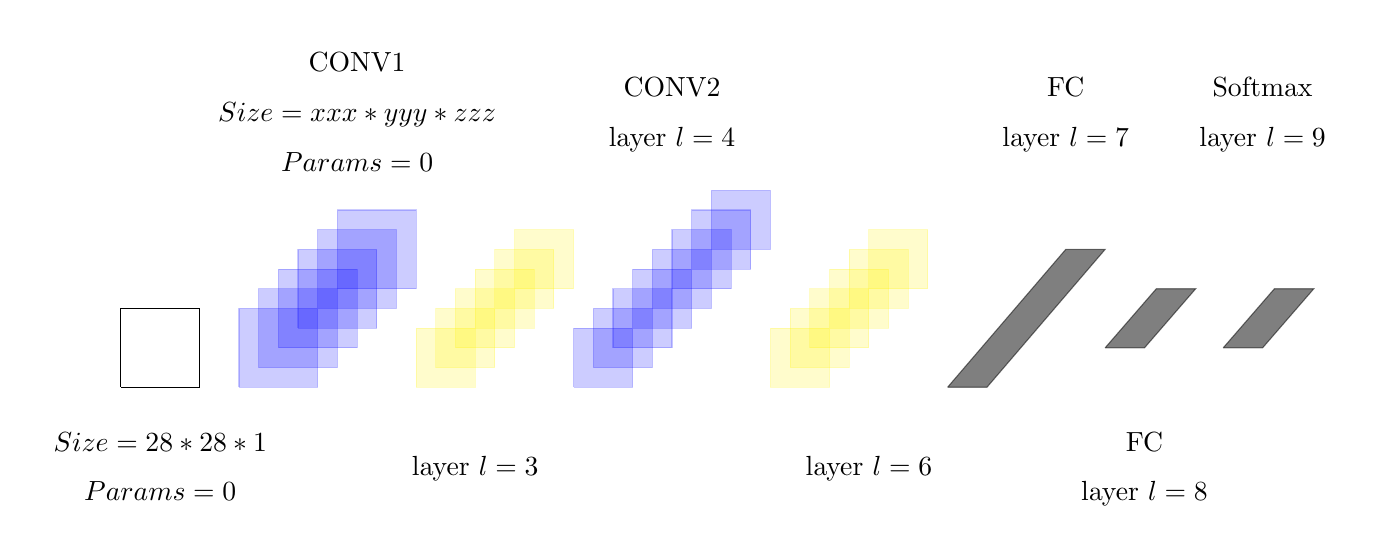
\begin{tikzpicture}
		\node at (0.5,-1){\begin{tabular}{c}$Size = 28 * 28 * 1$\\$Params = 0$\end{tabular}};
		
		\draw (0,0) -- (1,0) -- (1,1) -- (0,1) -- (0,0);
		
		\node at (3,3.5){\begin{tabular}{c}CONV1\\$Size = xxx * yyy * zzz$\\$Params = 0$\end{tabular}};
		
		\draw[fill=blue,opacity=0.2,draw=blue] (2.75,1.25) -- (3.75,1.25) -- (3.75,2.25) -- (2.75,2.25) -- (2.75,1.25);
		\draw[fill=blue,opacity=0.2,draw=blue] (2.5,1) -- (3.5,1) -- (3.5,2) -- (2.5,2) -- (2.5,1);
		\draw[fill=blue,opacity=0.2,draw=blue] (2.25,0.75) -- (3.25,0.75) -- (3.25,1.75) -- (2.25,1.75) -- (2.25,0.75);
		\draw[fill=blue,opacity=0.2,draw=blue] (2,0.5) -- (3,0.5) -- (3,1.5) -- (2,1.5) -- (2,0.5);
		\draw[fill=blue,opacity=0.2,draw=blue] (1.75,0.25) -- (2.75,0.25) -- (2.75,1.25) -- (1.75,1.25) -- (1.75,0.25);
		\draw[fill=blue,opacity=0.2,draw=blue] (1.5,0) -- (2.5,0) -- (2.5,1) -- (1.5,1) -- (1.5,0);
		
		\node at (4.5,-1){\begin{tabular}{c}layer $l = 3$\end{tabular}};
		
		\draw[fill=yellow,opacity=0.2,draw=yellow] (5,1.25) -- (5.75,1.25) -- (5.75,2) -- (5,2) -- (5,1.25);
		\draw[fill=yellow,opacity=0.2,draw=yellow] (4.75,1) -- (5.5,1) -- (5.5,1.75) -- (4.75,1.75) -- (4.75,1);
		\draw[fill=yellow,opacity=0.2,draw=yellow] (4.5,0.75) -- (5.25,0.75) -- (5.25,1.5) -- (4.5,1.5) -- (4.5,0.75);
		\draw[fill=yellow,opacity=0.2,draw=yellow] (4.25,0.5) -- (5,0.5) -- (5,1.25) -- (4.25,1.25) -- (4.25,0.5);
		\draw[fill=yellow,opacity=0.2,draw=yellow] (4,0.25) -- (4.75,0.25) -- (4.75,1) -- (4,1) -- (4,0.25);
		\draw[fill=yellow,opacity=0.2,draw=yellow] (3.75,0) -- (4.5,0) -- (4.5,0.75) -- (3.75,0.75) -- (3.75,0);
		
		\node at (7,3.5){\begin{tabular}{c}CONV2\\layer $l = 4$\end{tabular}};
		
		\draw[fill=blue,opacity=0.2,draw=blue] (7.5,1.75) -- (8.25,1.75) -- (8.25,2.5) -- (7.5,2.5) -- (7.5,1.75);
		\draw[fill=blue,opacity=0.2,draw=blue] (7.25,1.5) -- (8,1.5) -- (8,2.25) -- (7.25,2.25) -- (7.25,1.5);
		\draw[fill=blue,opacity=0.2,draw=blue] (7,1.25) -- (7.75,1.25) -- (7.75,2) -- (7,2) -- (7,1.25);
		\draw[fill=blue,opacity=0.2,draw=blue] (6.75,1) -- (7.5,1) -- (7.5,1.75) -- (6.75,1.75) -- (6.75,1);
		\draw[fill=blue,opacity=0.2,draw=blue] (6.5,0.75) -- (7.25,0.75) -- (7.25,1.5) -- (6.5,1.5) -- (6.5,0.75);
		\draw[fill=blue,opacity=0.2,draw=blue] (6.25,0.5) -- (7,0.5) -- (7,1.25) -- (6.25,1.25) -- (6.25,0.5);
		\draw[fill=blue,opacity=0.2,draw=blue] (6,0.25) -- (6.75,0.25) -- (6.75,1) -- (6,1) -- (6,0.25);
		\draw[fill=blue,opacity=0.2,draw=blue] (5.75,0) -- (6.5,0) -- (6.5,0.75) -- (5.75,0.75) -- (5.75,0);
		
		\node at (9.5,-1){\begin{tabular}{c}layer $l = 6$\end{tabular}};
		
		\draw[fill=yellow,opacity=0.2,draw=yellow] (9.5,1.25) -- (10.25,1.25) -- (10.25,2) -- (9.5,2) -- (9.5,1.25);
		\draw[fill=yellow,opacity=0.2,draw=yellow] (9.25,1) -- (10,1) -- (10,1.75) -- (9.25,1.75) -- (9.25,1);
		\draw[fill=yellow,opacity=0.2,draw=yellow] (9,0.75) -- (9.75,0.75) -- (9.75,1.5) -- (9,1.5) -- (9,0.75);
		\draw[fill=yellow,opacity=0.2,draw=yellow] (8.75,0.5) -- (9.5,0.5) -- (9.5,1.25) -- (8.75,1.25) -- (8.75,0.5);
		\draw[fill=yellow,opacity=0.2,draw=yellow] (8.5,0.25) -- (9.25,0.25) -- (9.25,1) -- (8.5,1) -- (8.5,0.25);
		\draw[fill=yellow,opacity=0.2,draw=yellow] (8.25,0) -- (9,0) -- (9,0.75) -- (8.25,0.75) -- (8.25,0);
		
		\node at (12,3.5){\begin{tabular}{c}FC\\layer $l = 7$\end{tabular}};
		
		\draw[fill=black,draw=black,opacity=0.5] (10.5,0) -- (11,0) -- (12.5,1.75) -- (12,1.75) -- (10.5,0);
		
		\node at (13,-1){\begin{tabular}{c}FC\\layer $l = 8$\end{tabular}};
		
		\draw[fill=black,draw=black,opacity=0.5] (12.5,0.5) -- (13,0.5) -- (13.65,1.25) -- (13.15,1.25) -- (12.5,0.5);

		\node at (14.5,3.5){\begin{tabular}{c}Softmax\\layer $l = 9$\end{tabular}};
		
		\draw[fill=black,draw=black,opacity=0.5] (14,0.5) -- (14.5,0.5) -- (15.15,1.25) -- (14.65,1.25) -- (14,0.5);
	\end{tikzpicture}
	\caption[Architecture of a traditional convolutional neural network.]{The architecture of the original convolutional neural network, as introduced by LeCun et al. (1989), alternates between convolutional layers including hyperbolic tangent non-linearities and subsampling layers. In this illustration, the convolutional layers already include non-linearities and, thus, a convolutional layer actually represents two layers. The feature maps of the final subsampling layer are then fed into the actual classifier consisting of an arbitrary number of fully connected layers. The output layer usually uses softmax activation functions.}
	\label{fig:traditional-convolutional-network}
\end{figure}

$
\text{size after applying convolution layer} = \left\lfloor \frac{n + 2p - f}{s} + 1 \right\rfloor
$

\subsection{1}


\end{latin}

%%%%%%%%%%%%%%%%%%%%%%%%%%%%%%%%%%%
%%%%%%%%%%%%%%%%%%%%%%%%%%%%%%%%%%%
%%%%%%%%%%%%%%%%%%%%%%%%%%%%%%%%%%%



\section*{منابع}
\renewcommand{\section}[2]{}%
\begin{thebibliography}{99} % assumes less than 100 references
%چنانچه مرجع فارسی نیز داشته باشید باید دستور فوق را فعال کنید و مراجع فارسی خود را بعد از این دستور وارد کنید


\begin{LTRitems}

\resetlatinfont

\bibitem{b1} https://www.shiksha.com/online-courses/articles/relu-and-sigmoid-activation-function/
\bibitem{b1} https://medium.com/@amanatulla1606/vanishing-gradient-problem-in-deep-learning-understanding-intuition-and-solutions-da90ef4ecb54
\bibitem{b1} https://en.wikipedia.org/wiki/Rectifier\_(neural\_networks)
\bibitem{b1} https://wandb.ai/ayush-thakur/dl-question-bank/reports/ReLU-vs-Sigmoid-Function-in-Deep-Neural-Networks--VmlldzoyMDk0MzI
\bibitem{b1} https://medium.com/swlh/why-are-neural-nets-non-linear-a46756c2d67f
\end{LTRitems}

\end{thebibliography}


\end{document}
